% definit le type de document et ses options
\documentclass[a4paper,12pt]{article}

% des paquetages indispensables, qui ajoutent des fonctionnalites
\usepackage[latin1]{inputenc}
\usepackage[T1]{fontenc}
\usepackage{amsfonts, amsmath, amssymb, amstext, latexsym,bm}
\usepackage{fullpage}
\usepackage{graphicx, epsifig}
\usepackage{url}
\usepackage{xspace}
\usepackage[francais]{babel}
% pour ecrire les reponses
\newtheorem{exercice}{Exercice}

% des commandes utiles pour ecrire des maths : rajoutez les votres!
\newcommand{\dx}{\,dx}
\newcommand{\ito}{,\dotsc,}
\newcommand{\R}{\mathbb{R}}
\newcommand{\N}{\mathbb{N}}
\newcommand{\Poly}[1]{\mathcal{P}_{#1}}
\newcommand{\abs}[1]{\left\lvert#1\right\rvert}
\newcommand{\norm}[1]{\left\lVert#1\right\rVert}
\newcommand{\pars}[1]{\left(#1\right)}
\newcommand{\bigpars}[1]{\bigl(#1\bigr)}
\newcommand{\set}[1]{\left\{#1\right\}}
\newcommand{\ind}{{{\large 1} \hspace*{-1.6mm} {\large 1}}}

% titre, auteur et date
\title{TP Principes et M\'{e}thodes Statistiques}
\author{Gabriel Sarrazin, Nejmeddine Douma, Simon Rabourg}
\date{Avril 2015}

% le debut du contenu
%===============
\begin{document}
%===============

% pour afficher titre, auteur et date
\maketitle



\section{Introduction}

TODO

\section{Analyse des d�fauts de cuves}

\begin{enumerate}

\item Les mesures des trois cuves pr�sentent des valeurs minimums assez proches les unes des autres: 2.007, 2.006 et 2.059. La cuve 2 poss�de la valeur maximale 5.437 et la variance la plus grande 0.54127686. Tandis que la cuve 1 s'empare du maximum des �cat-types 1.023202 et du maximum du coefficient de variation empirique 0.3563262. Les mesures de la cuve 3 pr�sentent le plus de r�gularit� avec le minimum de variation 0.15907528, le minimum d'�cart-type 0.4163554 et de coefficient de variation empirique 0.1475989 .

D'apr�s les allures des histogrammes des mesures de la cuve 1 (figures 1 et 2) et celles des mesures de la cuve 2 (figures 3 et 4), ces deux �chantillions sont vraisemblablement de loi exponentielle. Les figures 5 et 6 montrent que les mesures de la cuve 3 sont vraisemblalement de loi normale.

\begin{figure}
\centering
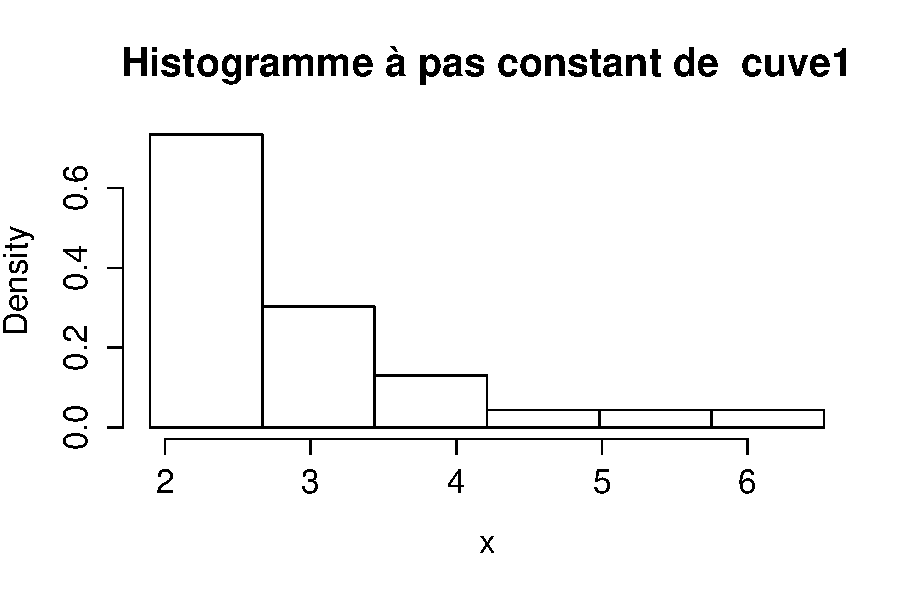
\includegraphics[width=1.0\textwidth]{figures/histopas_cuve1.pdf}
\caption{Histogramme � pas constant de cuve1 obtenu dans R}
\end{figure}

\begin{figure}[h]
\centering
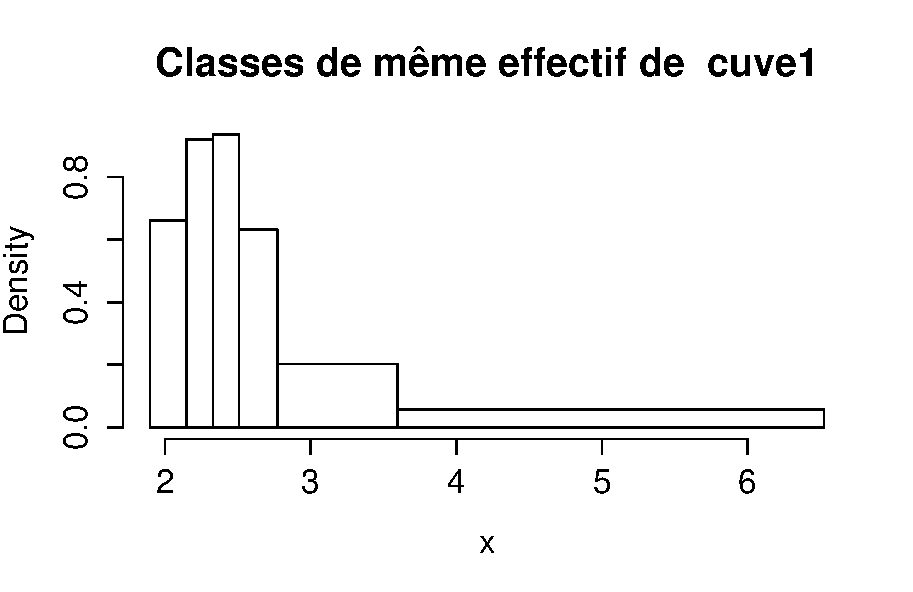
\includegraphics[width=1.0\textwidth]{figures/histoeff_cuve1.pdf}
\caption{Histogramme � classe de m�me effectif de cuve1 obtenu dans R}
\end{figure}

\begin{figure}[h]
\centering
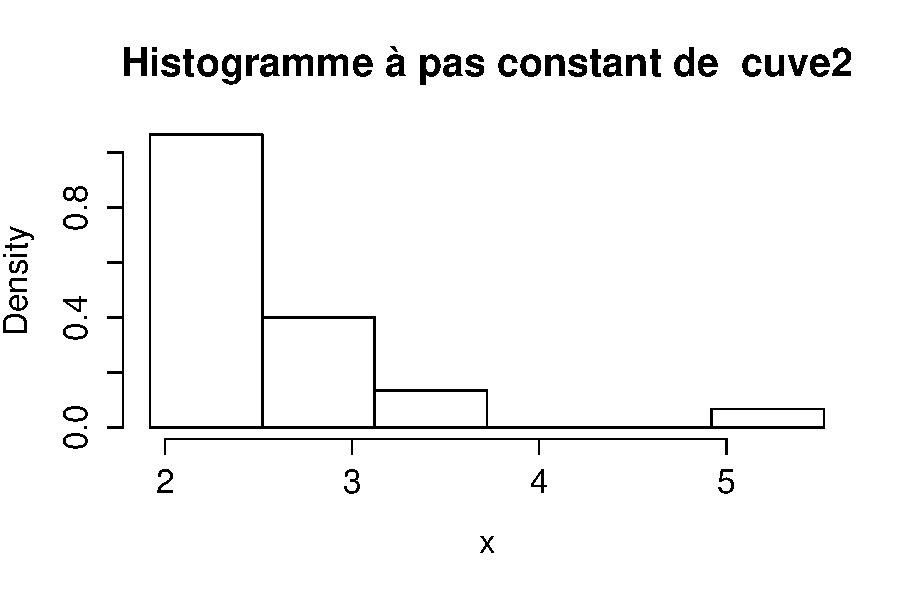
\includegraphics[width=1.0\textwidth]{figures/histopas_cuve2.pdf}
\caption{Histogramme � pas constant de cuve2 obtenu dans R}
\end{figure}

\begin{figure}[h]
\centering
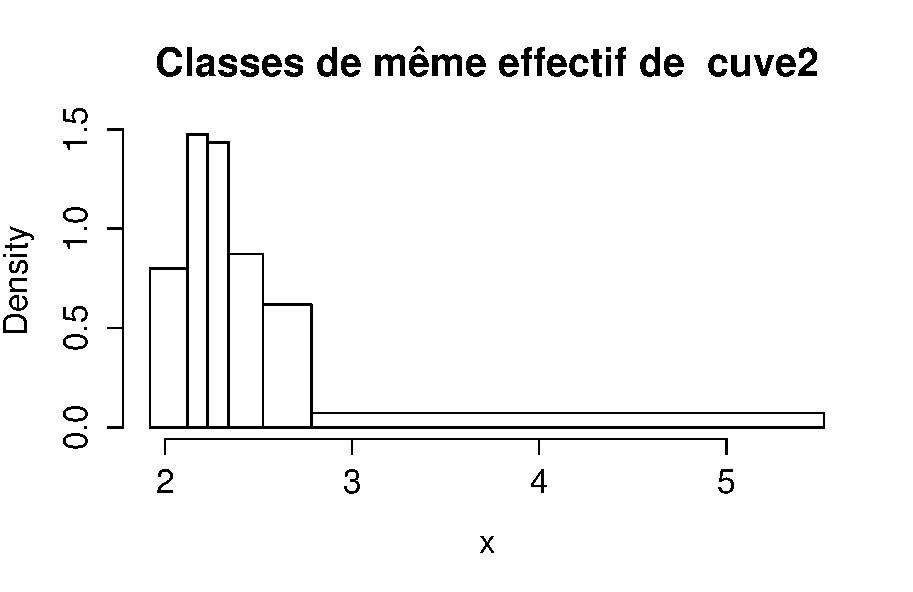
\includegraphics[width=1.0\textwidth]{figures/histoeff_cuve2.pdf}
\caption{Histogramme � classe de m�me effectif de cuve2 obtenu dans R}
\end{figure}

\begin{figure*}[h]
\centering
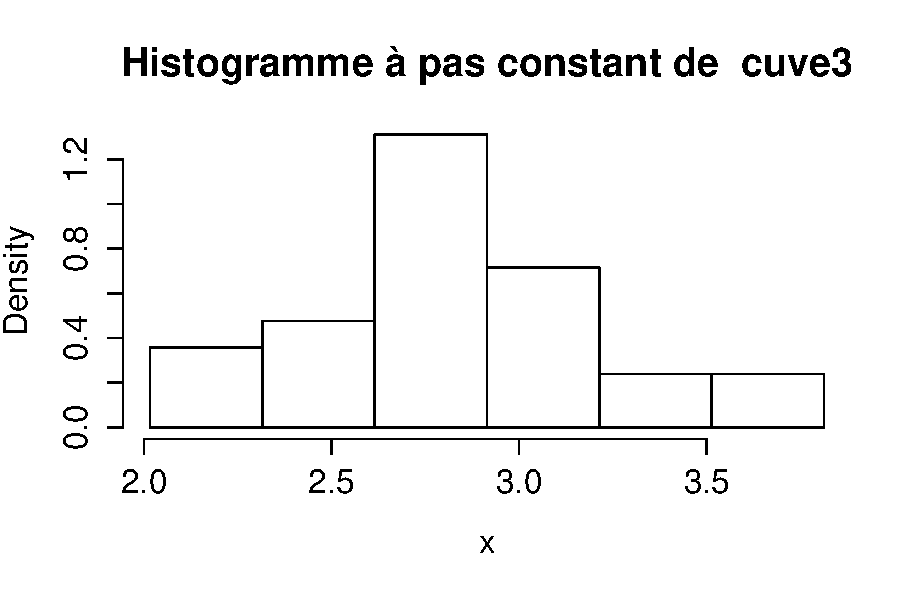
\includegraphics[width=1.0\textwidth]{figures/histopas_cuve3.pdf}
\caption{Histogramme � pas constant de cuve3 obtenu dans R}
\end{figure*}

\begin{figure*}[h]
\centering
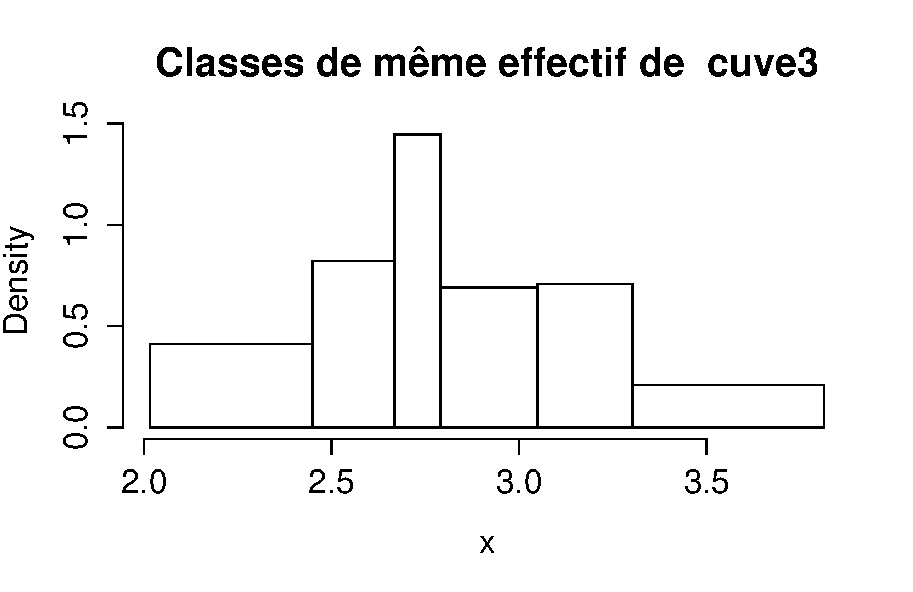
\includegraphics[width=1.0\textwidth]{figures/histoeff_cuve3.pdf}
\caption{Histogramme � classe de m�me effectif de cuve3 obtenu dans R}
\end{figure*}





\vspace{3mm}


\item Caculons $F_x$ la fonction de r�partition de $X$.

$X$ est une variable al�atoire de loi ${\cal P}a(a, 2)$,  sa densit� est :
$ f(x) = \frac{a \, 2^a}{x^{1+a}} \, \ind_{[2,+\infty[}(x)$, donc


$ \begin{array}{lcl}
$$F_x(x)$$ &  $$=$$ & $$ \int_{-\infty}^{x} \frac{a \, 2^a}{t^{1+a}} \, \ind_{[2,+\infty[}(t) \, \mathrm dt $$ \\
 &  $$=$$ & $ \left\{ \begin{array}{l l}  $$\int_{2}^{x} a  2^a \, t^{-(1+a)} \, \mathrm dt $$ & si $$\, x > 2 $$ \\ 0 & sinon. \\\end{array} \right. $ & \\
 $$F_x(x)$$ &  $$=$$ & $\left\{ \begin{array}{l l}   $$1 - 2^a \, x^{-a} $$ & si $$ x > 2 $$ \\ 0 & sinon. \\\end{array} \right. $ & \\
\\
\end{array}$

\vspace{3mm}

Le th�or�me de transfert donne:

$
\begin{array}{lcl}
$$\bm{ \mathbb{E}}[X]$$ &  $$=$$ & $$\int_{-\infty}^{+\infty} t\, \frac{a \, 2^a}{t^{1+a}} \, \ind_{[2,+\infty[}(t) \, \mathrm dt $$ \\
 & $$=$$ & $$ \frac{a2^a}{1-a}  \, [x^{1-a} ]_2^{+\infty} $$  \\
\\
\end{array}
$

$
\begin{array}{lcl}
$$Var(X)$$ &  $$=$$ & $$ \bm{ \mathbb{E}}[X^2] - \bm{ \mathbb{E}}[X]^2  $$ \\
 & $$=$$ & $$ {\frac{a2^a}{2-a}  \, [x^{2-a} ]_2^{+\infty} }  -  ({\frac{a2^a}{1-a}  \, [x^{1-a} ]_2^{+\infty} })^2 $$  \\
\\
\end{array}
$

Pour que  $\bm{ \mathbb{E}}[X]$ et Var(X) soit finis il faut que a $\geq$ 2.



\item Caculons $F_Y$ la fonction de r�partition de $Y=\ln {\dsp \frac{X}{2}}$.

$ \begin{array}{lcl}
$$F_Y(x)$$ &  $$=$$ & $$  \bm{ \mathbb{P}}( Y < x )  $$ \\
 &  $$=$$ & $$\bm{ \mathbb{P}}(\ln {\dsp \frac{X}{2}} < x )  $$ \\
 &  $$=$$ & $$\bm{ \mathbb{P}}(\ln X - \ln 2  < x ) $$ \\
 &  $$=$$ & $$\bm{ \mathbb{P}}(X  < \exp ( x + \ln 2) ) $$ \\
 &  $$=$$ & $$\bm{ \mathbb{P}}(X  < 2\exp(x) ) $$ \\
 &  $$=$$ & $$ F_X(2\exp(x))$$ \\
 &  $$=$$ & $  \left\{ \begin{array}{l l}  $$ 1 - 2^a (2\exp(x))^{-a} $$ & si $$\, x > 2 $$ \\ 0 & sinon. \\\end{array} \right. $ \\
$$F_Y(x)$$  &  $$=$$ &  $  \left\{ \begin{array}{l l}  $$ 1 - \exp(-ax) $$  & si $$\, x > 2 $$ \\ 0 & sinon. \\\end{array} \right. $ \\
\\
\end{array} $

Donc Y suit la loi $\cal{E}$(a).

\vspace{3mm}

\item Trouvons une fonction pivotale pour d�terminer l'expression d'un intervalle de confiance de seuil $\alpha$ pour a.
On a besoin des trois lemmes suivant:


Lemme 1: Si $\lambda$>0, $\mu$ >0 et  $X$ une variable al�atoire r�elle de loi $\cal{E}$($\lambda$) alors $\mu X \sim  \cal{E}(\frac{\lambda}{\mu}) $

Lemme 2: Si $X_1, X_2, ... , X_n$ une famille de variables al�atoires r�elles ind�pendantes et identiquement distriu�es de loi  $\cal{E}$($\lambda$) alors $\sum_{i=0}^{n}X_i \sim \Gamma ($n,$\lambda)$.

Lemme 3: $\Gamma ($n, $\frac{1}{2}$) et $\chi_{2n}^{2}$ d�crivent la m�me loi de probabilit�.

 Soit $Y_1, Y_2, ... , Y_n$ une famille de variables al�atoires r�elles ind�pendantes et identiquement distriu�es de loi  $\cal{E}$(a). 
$2aY_1, 2aY_2, ... , 2aY_n$ sont donc de loi $ \cal{E}$($\frac{1}{2}$) (Lemme 1).
D'o�, 2a$\sum_{i=0}^{n}Y_i \sim \Gamma ($n,$\frac{1}{2})$ (Lemme 2).
Donc, 2a$\sum_{i=0}^{n}Y_i \sim \chi_{2n}^{2}$.
Or $\chi_{2n}^{2}$ ne d�pend pas du param�tre a, donc 2a$\sum_{i=0}^{n}Y_i$ est une fonction pivotale.

En notant $z_{n,\alpha}$ 1-($\alpha$)-quantile de la loi $\chi_{2n}^{2}$ on a:

$$ \bm{ \mathbb{P}}( z_{2n,1-\frac{\alpha}{2}} \leq   2a\sum_{i=0}^{n}Y_i \leq  z_{2n,\frac{\alpha}{2}} ) = 1 - \frac{\alpha}{2} - \frac{\alpha}{2} = 1-\alpha $$

D'o�:

$$ \bm{ \mathbb{P}}(\a \in [\frac{z_{2n,1-\frac{\alpha}{2}} }{ 2a\sum_{i=0}^{n}Y_i}, \frac{ z_{2n,\frac{\alpha}{2}}}{ 2a\sum_{i=0}^{n}Y_i}]) = 1-\alpha $$

Donc:

$ [\frac{z_{2n,1-\frac{\alpha}{2}} }{ 2a\sum_{i=0}^{n}Y_i}, \frac{ z_{2n,\frac{\alpha}{2}}}{ 2a\sum_{i=0}^{n}Y_i}] $ est un intervalle de confiance de seuil $\alpha$ pour a





\end{enumerate}



% fin du document
%=============
\end{document}
%=============

